\chapter{Configurable Timed CEGAR} \label{chap:timed_cegar}

%In this section an approach of applying CEGAR to the timed automaton is explained. Some details of implementation are also discussed.

  
\section{Algorithms}

\todo{Algoritmusok, leírással, hol használják, hogyan lehet TA-ra alkalmazni, miért jó, stb. + hogyan fog beleilleszkedni a konfigurálható izébe (milyen dobozok)}

\subsection{Adapted algorithms}

\subsection{Solver-based approaches}

\subsection{Statespace refinement}

\subsection{Trace Activity}


\section{Architecture}

\subsection{Overview}

\todo{CEGAR dobozok, interfészek, cserélgethetőség, stb. ábrával } 

\subsection{Modules}

\todo{Elkészült dobozok, intefészek, kombinálhatóság}

%\section{}

%\section{Introducing a new algorithm}

%\todo{El kéne nevezni ezt az algoritmust és akkor nem kellene mindenhol "az X. fejezetben bemutatt algoritmus"-ként hivatkozni rá.}

%My algorithm is explained in this section. To ease understanding it is also demonstrated on the automaton in Figure \ref{fig:loopinfinite}, with the error location being the location $end$.

%\subsection{Overview}

 %Due to these disadvantages discussed above I have decided that my approach of applying CEGAR to the reachability analysis of timed automata will modify the reachability algorithm instead of using it as a black box module. My approach applies abstraction to the zone graph of the automaton, instead of the automaton itself. The reachability algorithm (which will now be a CEGAR-based algorithm) will refine the zone graph iteration by iteration until reachability can be decided. The CEGAR loop is interpreted the following way.

 %\begin{description}
 %	\item[Initial abstraction] The key problem about constructing the initial abstraction of the zone graph is that the zone graph is unknown so the abstraction has to be derived from the automaton itself. The idea is really simple: just like the other approaches I also use the location graph of the automaton as the initial abstraction, except in my algorithm it is considered to be the abstraction of the zone graph, not the automaton. To create an overapproximation of the zones, we simply consider every valuations to be reachable in all locations. The zone containing all valuation is denoted by $z_\infty$.
 %	\item[Model checking] Since the abstract zone graph is an abstraction of the reachability graph, model checking becomes a pathfinding problem in the current abstraction of the zone graph. The error location is either proven unreachable or a new trace (path in the graph) is found from the initial node to the target node.
 %	\item[Analysis] This part is about finding out if the error location is really reachable on the trace found in the model-checking phase. The way to do that is by finding out how this path of the abstract zone graph would look like in the refined (real) zone graph. This can be achieved by using the reachability algorithm, but only for the given trace. As discussed in Section \ref{sec:reach}, because of the operation \emph{split} sometimes the real zone graph can branch, which means that the result of the simulation may be a tree instead of a simple path. Nevertheless, it is still easy to decide whether the counterexample is valid: if the error location could be reached by the path (on any branch), then the counterexample is valid. Otherwise, simulation will stop somewhere, typically because one of the transitions (on each branch) is not enabled. In this case the counterexample is spurious.
 %	\item[Refinement] In order to avoid the discussed disadvantages, this algorithm stores as many information of the analysis phase as it can - by replacing the counterexample trace in the abstraction of the zone graph with the calculated subgraph (tree) -- thus refining the abstraction.
 %\end{description}

 
 %\begin{figure} [h]
 %	\centering
 %	\begin{minipage} {0.2\linewidth}%
% 		\vspace*{10pt}%
% 		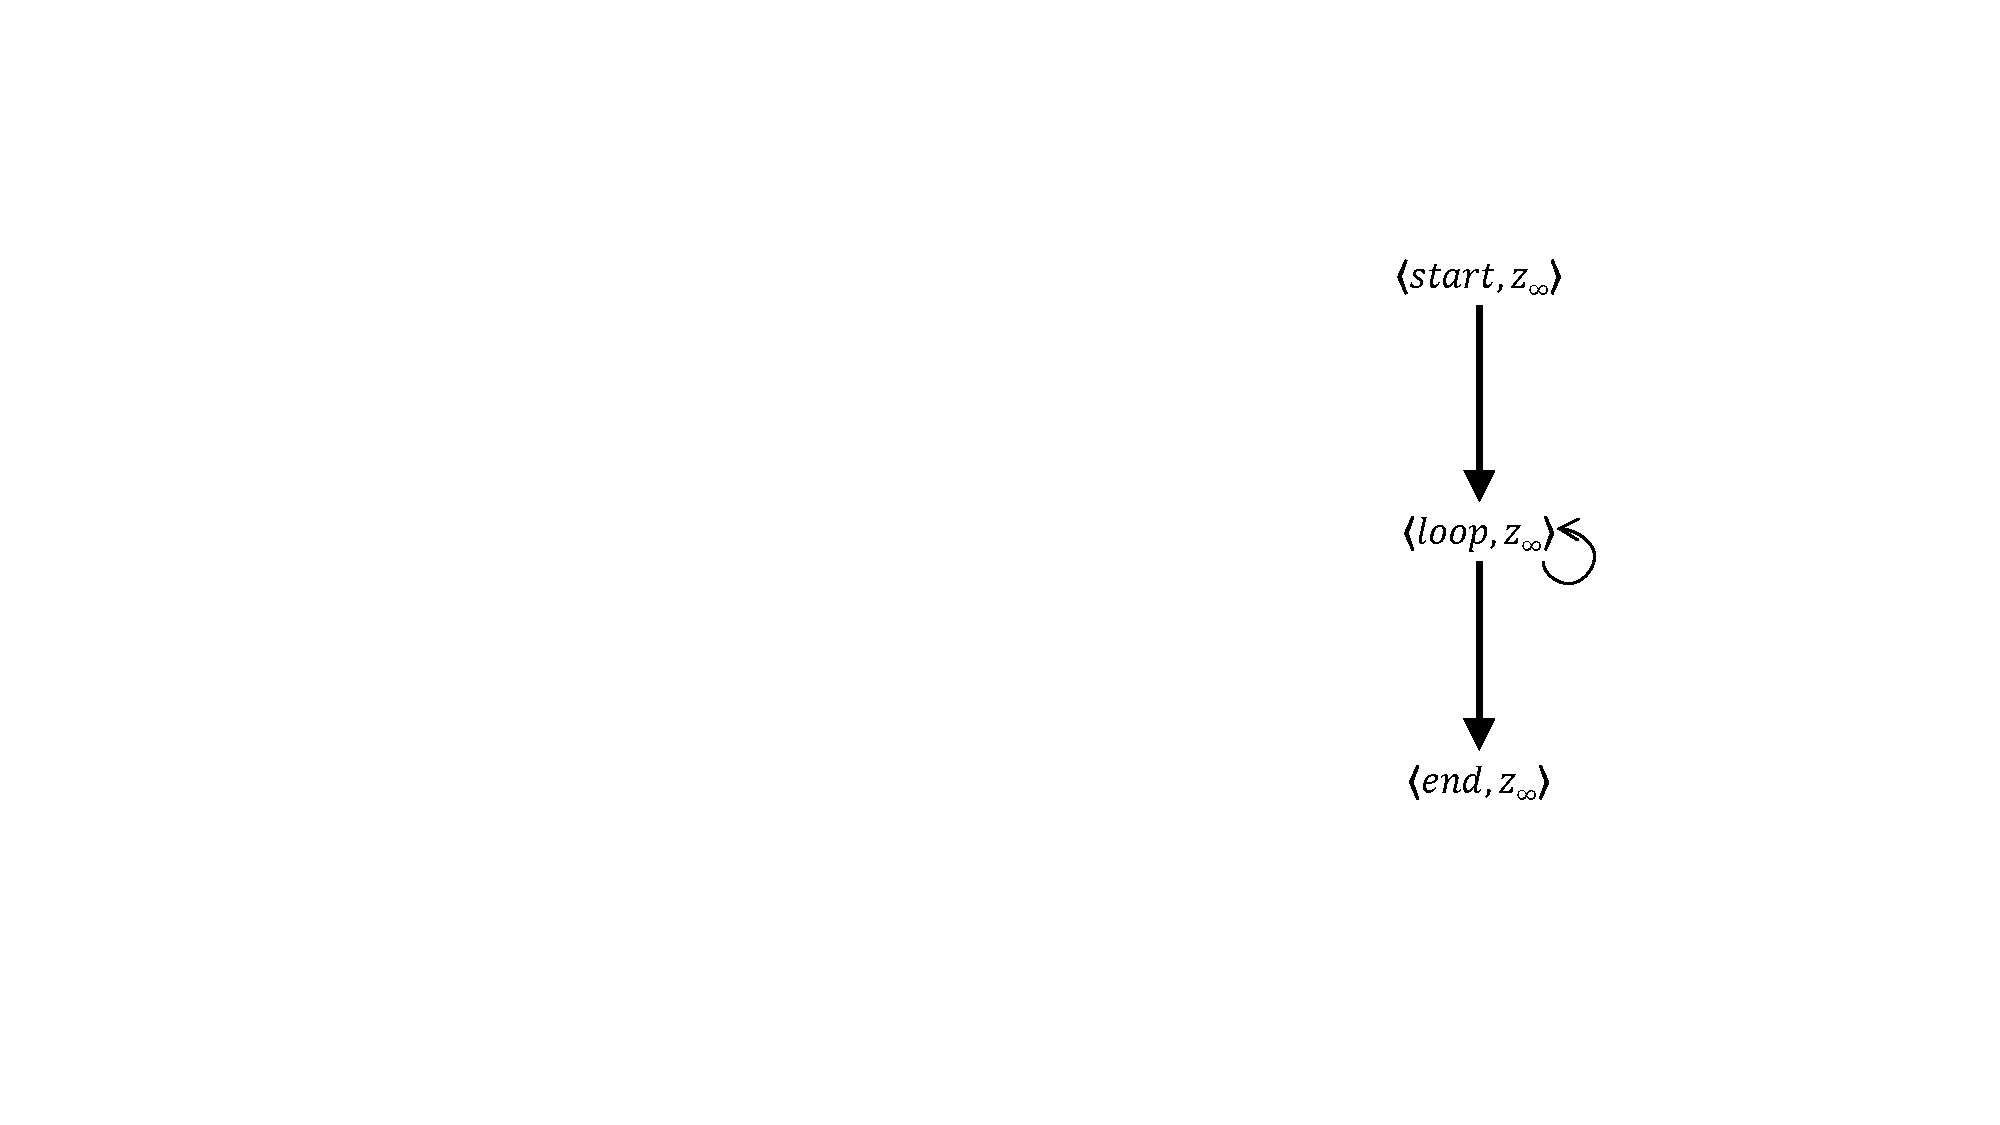
\includegraphics [width=\textwidth]{include/figures/loop_initial_abst}%
% 		\caption{Initial abstraction}
% 		\label{fig:x}
% 	\end{minipage}%
% 	\hspace{20pt}	%
% 	\begin{minipage} {0.2\linewidth}%
% 		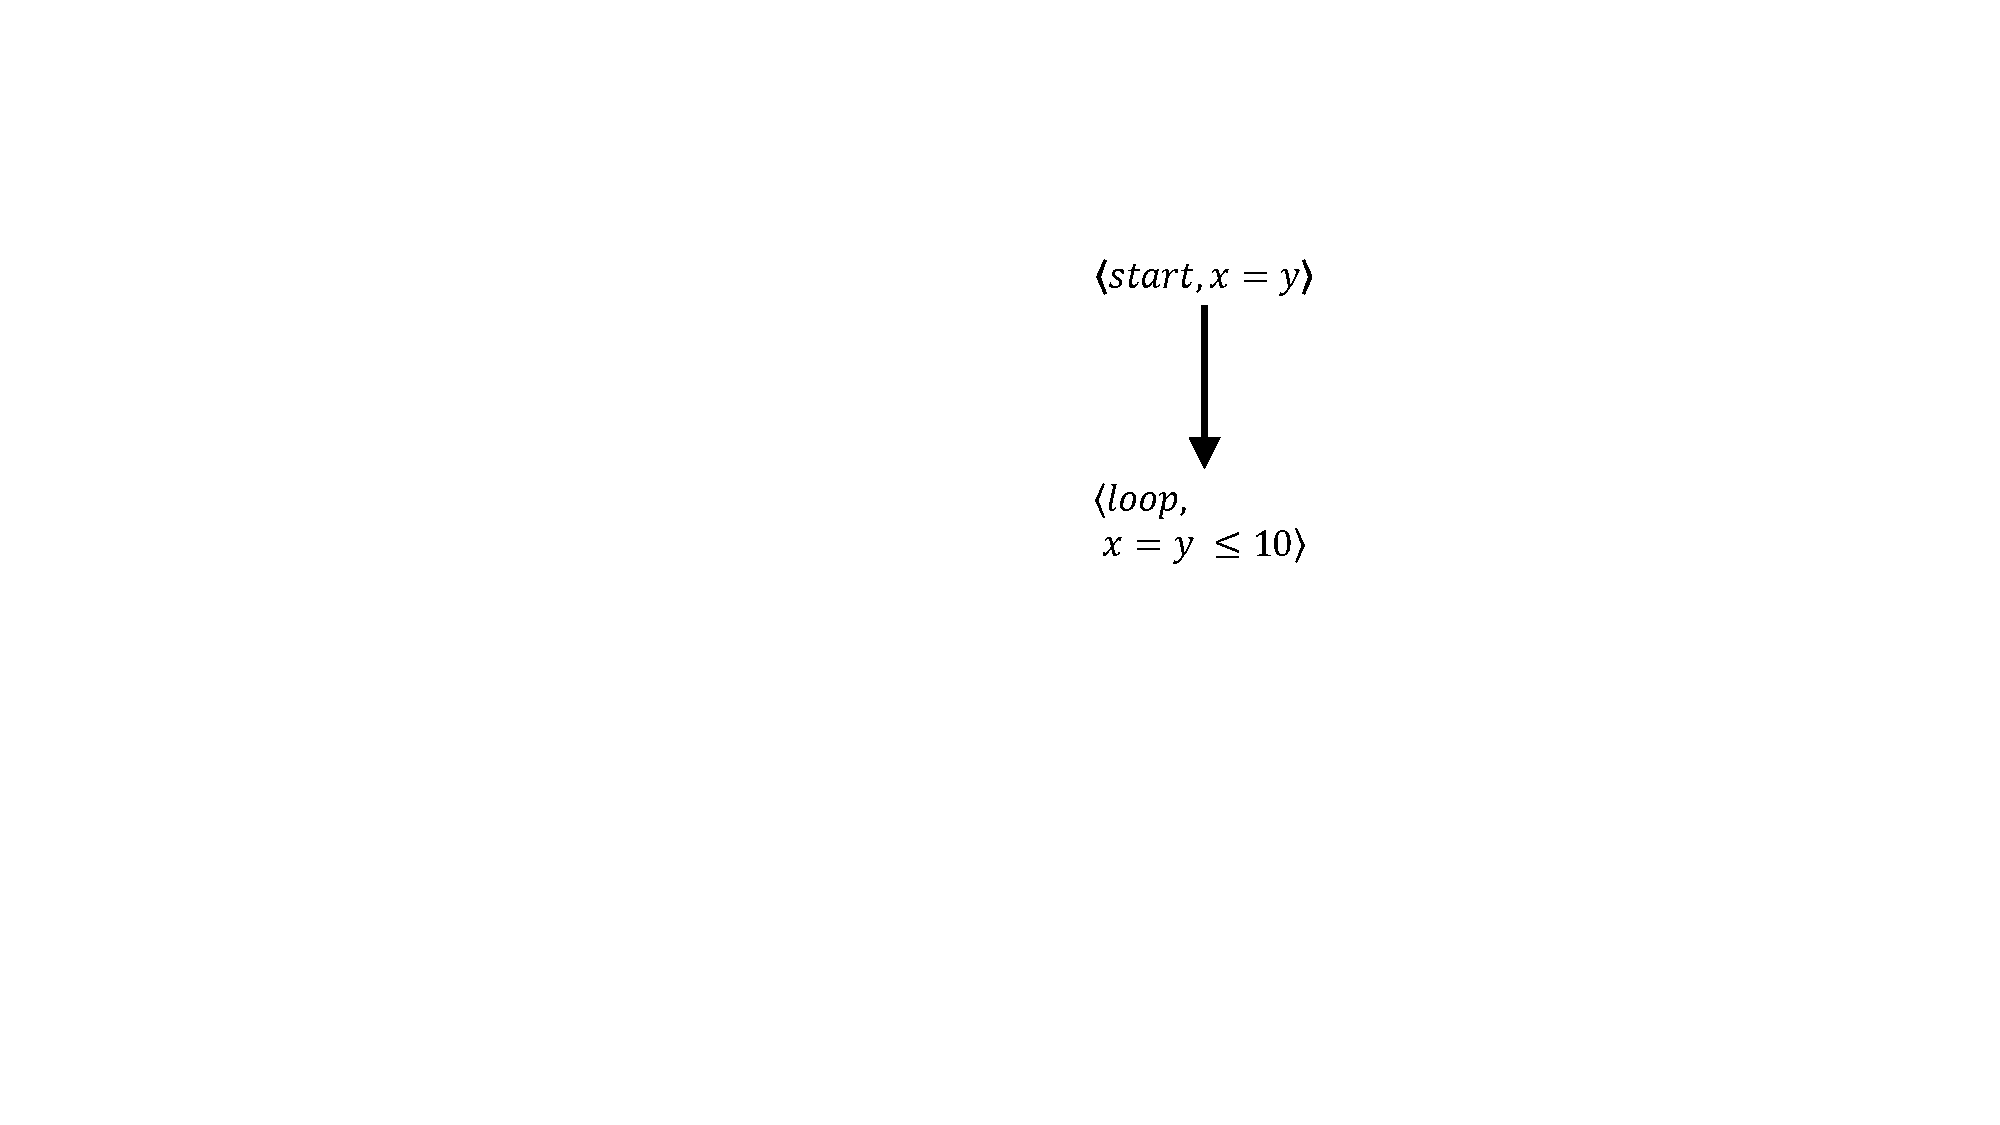
\includegraphics [width=\textwidth] {include/figures/loop_first_ref}%
% 		\vspace*{103pt}%
% 		\caption{Result of analysis}
% 		\label{fig:loopanal}
% 	\end{minipage}%
% 	\hspace{20pt}%
% 	\begin{minipage} {0.25\linewidth}%
% 		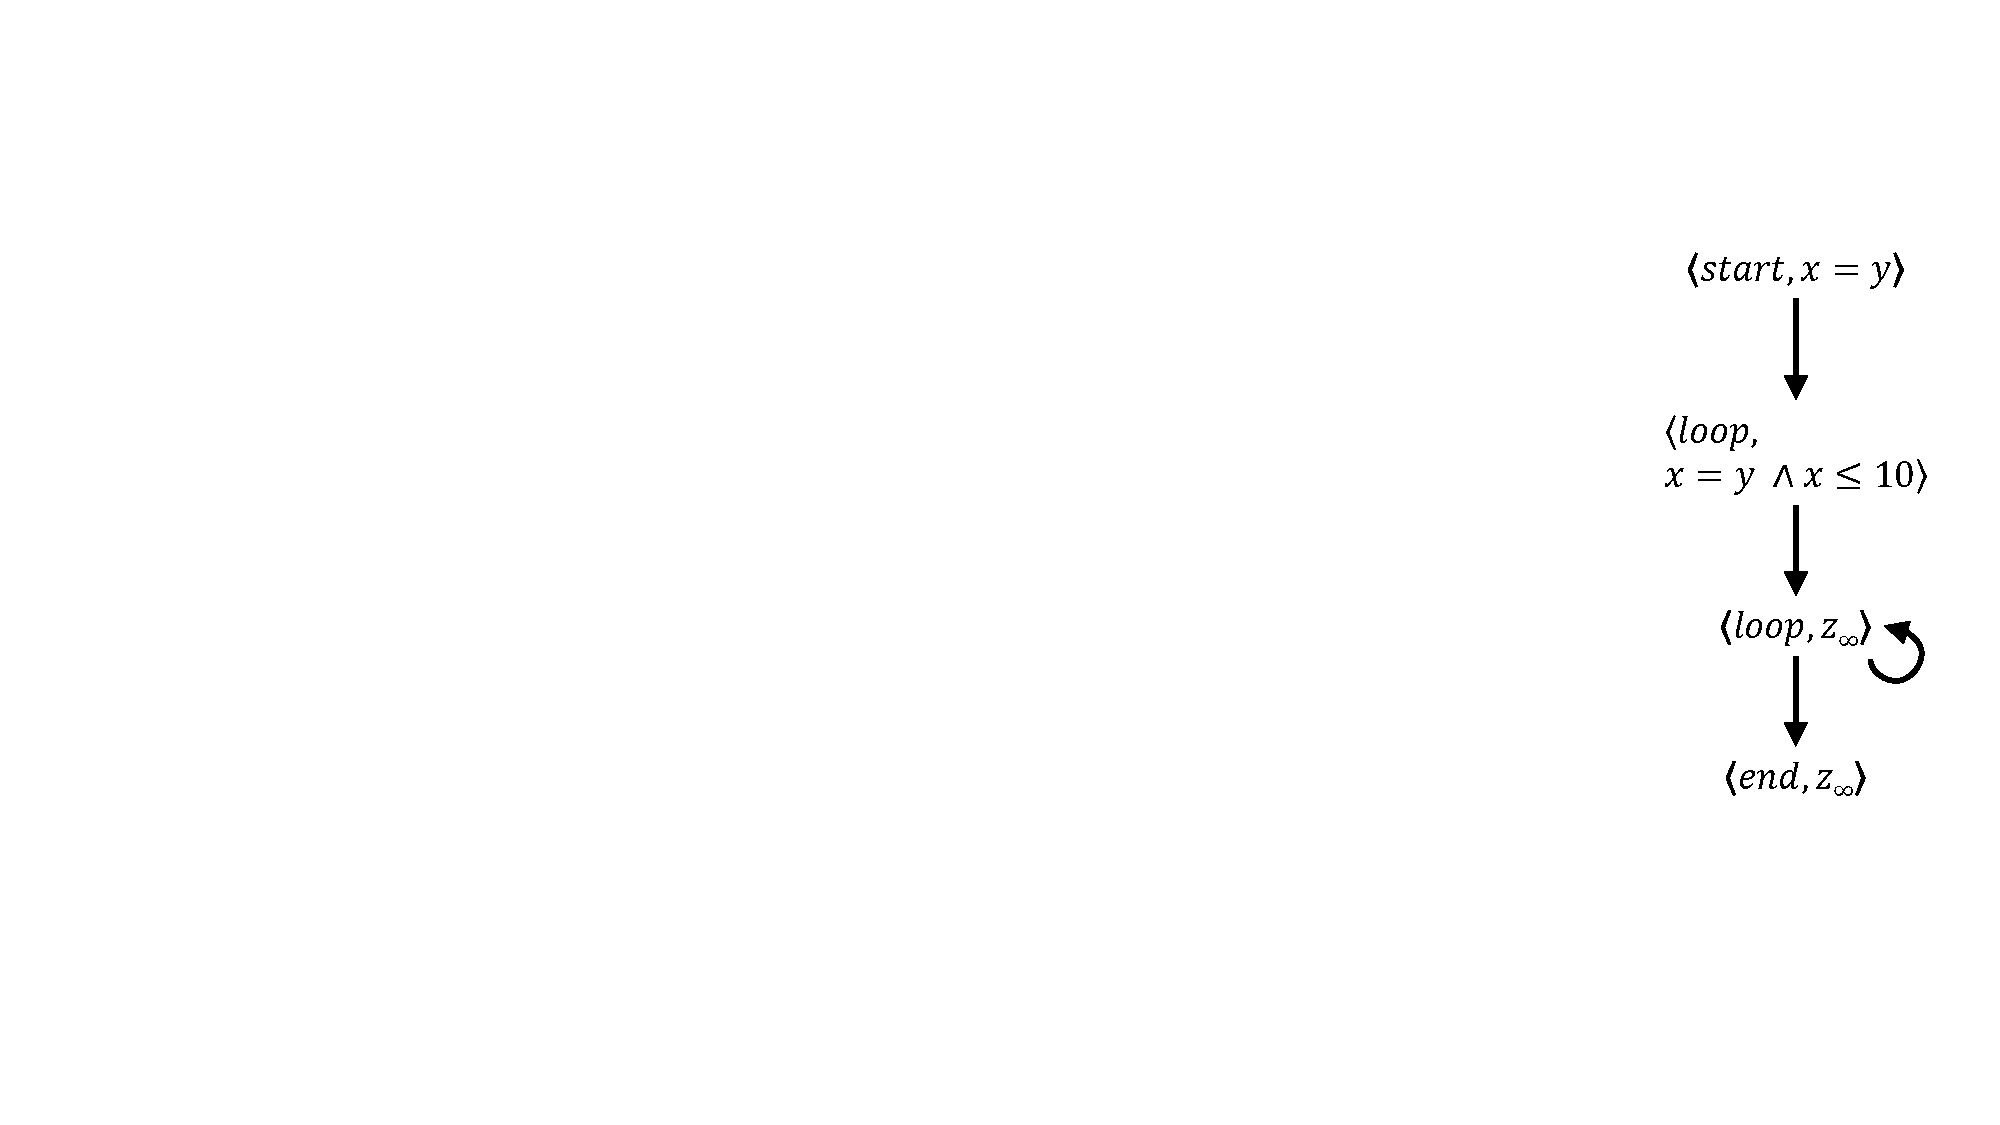
\includegraphics [width=\textwidth] {include/figures/loop_first_abst}%
% 		\vspace*{5pt}%
% 		\caption{After refinement}
% 		\label{fig:loopref}
% 	\end{minipage}
% 	\caption{Timed CEGAR on an example}
% \end{figure}
% 
 
%\subsection{Details}
%
%It is very important to perform the presented operations correctly. This section explains the algorithm step by step, demonstrating it on the example automaton in Figure \ref{fig:loopinfinite}.
%
%Constructing the initial abstraction is very straightforward: each node of the location graph are to be completed with the zone $z_\infty$. After that, model checking is simply a pathfinding in the current abstraction of the zone graph.
%
%\begin{example}
%	The initial abstraction of the example automaton's zone graph is depicted in Figure \ref{fig:x}. The first counterexample is denoted with bold arrows.
%\end{example}
%
%Simulation of the counterexample is performed by constructing the relevant part of the real zone graph. In the first iteration each node on the path will contain $z_\infty$. In this case, refinement starts from the node that belongs to the initial location and the refined zone is calculated as the initial zone of the zone graph.
%
%The result of pathfinding in the graph in Figure \ref{fig:x} is denoted by bold arrows. In case of the later iterations the first few nodes of the
%trace will already be refined, so the refinement can start from the first
%abstract node. The reachable zone should be calculated from the last refined zone,
%considering the guards and the reset as when constructing the zone graph.
%
%When the result of the refinement is more than one zone, the node on the path (and the edge pointing
%to it) is replicated, and one of the refined zones are assigned
%to each resulting node. The refinement can be continued from any of these nodes -- the path branches.
%All of these branches should be analyzed (refined) one by one.
%
%If the erroneous location is reachable through this path, the procedure finds it,
%and the CEGAR algorithm terminates. Otherwise, at some point a guard or a target invariant
%is not satisfied -- the transition is not enabled. The corresponding edge is removed and the analysis of the path terminates.
%
%\begin{example}
%	Consider the example. Since it is the first iteration, we start by constructing the initial node, $\langle start, x=y \rangle$. After that we calculate the next node on the trace $\langle loop, x=y \leq 10 \rangle$. When constructing the zone graph, we continued with the transition represented by the loop-edge but this time we only have to explore the zone graph through the transitions in the counterexample. The next transition is the transition represented by the edge directed to node $\langle end, z_\infty \rangle$. This transition is not enabled in the previously calculated zone, which means the counterexample is spurious. The resulting subgraph of the zone graph is depicted in Figure \ref{fig:loopanal}.
%\end{example}
%
%The goal of refinement is to eliminate the spurious counterexample from the abstract representation. Refinement is applied by replacing the abstract counterexample with the subgraph of the real zone graph calculated in the \emph{Analysis} phase. This operation has to be performed very carefully.
%
%Consider e.g. that the node in the abstract graph that is about to get replaced by one (or more) nodes in the subgraph has other incoming edges than the one in the counterexample. Since it is unknown what states are reachable in the location by the other incoming edges, the node can't be removed. Except, the edge representing the transition in the counterexample has to be redirected to the node with the calculated zone (if there are multiple nodes, it has to be replicated).
%
%Let us suppose that the graph is prepared to place the new node(s). To avoid wasting memory it is advised to use already refined zones in the graph. If the refined zone $z$ of the node $\langle l,z \rangle$ is a subzone of a zone $z'$ in a node $\langle l,z' \rangle$ (both nodes
%contain the same location $l$), then any state that is reachable from $\langle l,z \rangle$ is also reachable from $\langle l,z' \rangle$, thus there is no need to add  $\langle l,z \rangle$ to the graph. Instead, any edge leading to  $\langle l,z \rangle$ should be redirected to $\langle l,z' \rangle$. After that the replacement of the path can not continue from that $\langle l,z' \rangle$, since there might be more states reachable from $\langle l,z' \rangle$ than from $\langle l,z \rangle$. The remaining of the refined zones have to be recalculated and then the replacement can continue.
%
%When replacing the node, the outgoing edges should also be considered. The calculated subtree of the real zone graph only contained the edges in the trace, but in the abstract zone graph there are other outgoing edges of the node. These edges are the outgoing edges of the original (abstract) node in the zone graph, and they have to be replicated, as outgoing edges from the added node(s). After this we can continue with the next node.
%
%\begin{example}
%In the example replacing the initial node can simply be performed by replacing the zone $z_\infty$ with the zone $x=y$. On the other hand, replacing the node $loop$ has to be performed carefully. Since the loop-edge is an incoming edge of the node and is not part of the counterexample, the node can not be replaced. Instead, the incoming edge on the trace is redirected to the new node (in other words, the one to the original node is removed). Since a new node is added, we have to think about it's outgoing edges that are not on the trace -- in this case the only one is the loop edge. For reasons explained before, the loop edge has to be redirected to the abstract version of the node. Thus, the refinement is finished, and now the counterexample is eliminated from the abstract zone graph. Th resulting graph is depicted in Figure \ref{fig:loopref}.
%\end{example}
%
%
%%\section{Realization}
%
%%\todo{Megvalósítós részek ide + pszeudokód}
%
%\section{Evaluation}
%
%It is important to prove that the algorithm is correct, and that it terminates. Both proof relies on that of the original algorithm.
%
%The algorithm always terminates, because the abstraction of zone graph gets refined in every iteration. Even at worst case, the algorithm stops when the zone graph is completely refined.
%
%The algorithm is correct, because the original algorithm is correct. If the algorithm finds a counterexample, it is a trace in the original algorithm. Otherwise, if there is a counterexample in the original algorithm, this algorithm finds it at some point.
%
%
%
%%\todo{Terminálódás, komplexitás, stb.}
